\documentclass[../Bachelorarbeit.tex]{subfiles}
\begin{document}
\chapter{Stand der Technik}
\label{chap:analyse}

Nachdem in Kapitel \ref{chap:einfuehrung} - \nameref{chap:einfuehrung} die ersten konkreten Überlegungen bis hin zu einem \nameref{sec:anwendungsszenario} aufgezeigt wurden um den Inhalt und die Funktionsweise des Prototypen zu umreißen, widmet sich dieses Kapitel der Domäne für die der Prototyp entwickelt wird.\\
\\
Das Ziel besteht darin, einen kurzen Einblick auf die im Internet verfügbaren Service zu erhalten, welche sich auf die geografische Visualisierung von Daten spezialisiert haben. 
Neben dem Mehrwert, einen Überblick  zu erhalten, sollen speziell die Details und die Umsetzung der Online Dienste betrachtet werden.
Diese Erkenntnisse können für die spätere Entwicklung  des Konzeptes als wertvolle Informationen dienen.\\
\\
Der Schwerpunkt bei der Analyse der bestehenden Konzepten wurde auf Applikationen gelegt, welche in einem Webbrowser ausgeführt werden können, ohne weitere Software installieren zu müssen.
Diese Kriterien wurden definiert da sie am besten das Szenario mit der Außendienstplanung widerspiegeln, welches im Prototyp implementiert werden soll.\\
\\
Die getätigten Aussagen über die Webseite beziehen sich, wenn nicht anders erwähnt, auf den Stand von Sommer 2016 und behandeln jeweils die Ansicht in dem Desktop-Webbrowser Google Chrome.


\begin{comment}
Nachdem in Kapitel \ref{chap:einfuehrung} - \nameref{chap:einfuehrung} die ersten konkreten Überlegungen bis hin zu einem \nameref{sec:anwendungsszenario} aufgezeigt wurden um den Inhalt und die Funktionsweise des Prototypen zu umreißen, widmet sich dieses Kapitel der Domäne für die der Prototyp entwickelt wird.
Für diesen Zweck ist das Kapitel in zwei Abschnitte unterteilt. 
Im ersten Abschnitt (\nameref{chap:analyse:sec:sota}) wird ein Blick auf die Forschung und Fachliteratur geworfen, während sich der zweite Abschnitt (\nameref{chap:analyse:sec:analyBestehendeKonz}) mit echten Projekten beschäftigt, die eine Relevanz für den Prototypen darstellen.

\section{Literaturrecherche}
\label{chap:analyse:sec:sota}


\ideas{Einführung Themen aus der Entscheidungstheorie...Einzelne Punkte von Tufte, je nach Relevanz...Literaturrecherche ... sowie was aktueller Stand der Technik sowie Forschung.}



\section{Analyse von bestehenden Konzepten}
\label{chap:analyse:sec:analyBestehendeKonz}
\end{comment}




\section{Google Maps}
\label{chap:analyse:sec:sota:sec:google_maps}
Google Maps\footnote{
	Google Maps ist unter der Adresse https://www.google.at/maps/ zu erreichen. 
} ist mit einer Milliarde User im Monat (Stand 2012) wahrscheinlich der verbreitete Online-Kartendienst im Internet (vgl. \cite{McClendonGoogleMapsBlog} und \cite{McClendonYoutube}).  
Neben der Routenplanung mit Echtzeitdaten über das Verkehrsaufkommen bietet Google Maps auch die Funktionalität IN DER NÄHE an.
Mit dieser Funktion lassen sich Orte anhand eines Suchbegriffes, wie beispielsweise Pizzeria, oder mittels vordefinierter Kategorien, wie zum Beispiel Restaurant, in der zuvor definierten Umgebung oder Stadt finden.


\subsection{Aufbau von Google Maps}
Die Darstellung von Google Maps ist optisch in zwei Teile unterteilt.
Zum einen in die ausblendbare linke Seite, welche wiederum in die Bereiche \nameref{gmapsSearch} sowie die \nameref{gmapsList} der Ergebnisse unterteilt ist und zum anderen der größere rechte Teil, mit der\nameref{gmapsMap} (siehe Abb.: \ref{fig:googlemapOverview}).
Durch die blaue Hintergrundfarbe wird das \nameref{gmapsSearch} optisch von der \nameref{gmapsList} der Ergebnisse abgegrenzt.


\paragraph{Suchfeld}
\label{gmapsSearch}
Die Ansicht des Bereichs \nameref{gmapsSearch} kann der Abb.: \ref{fig:googlemapOverview}-1 entnommen werden.
Das Suchfeld stellt das zentrale Auswahlelement in Google Maps da. 
Neben dem eigentlich Textfeld, wurde an dieser Stelle auch ein Button integriert, mit dessen Hilfe ein weiteres Menü erscheint. 
Dieses Menü wird verwendet, um weitere Informationen  in der Karte ein- oder auszublenden, wie Beispielsweise die aktuelle Verkehrslage, oder allgemeine Optionen von Google Maps anzupassen wie unter anderem die Sprache.
Bei der eigentlichen Interaktion mit dem Suchfeld steht eine Unterstützung in Form einer Textvervollständigung zu Verfügung. 

\paragraph{Listendarstellung}
\label{gmapsList}
\nameref{fig:googlemapOverview} entnommen werden und wird durch den roten Rahmen mit der Nummerierung 2 markiert (links).
Dieser Bereich wird für die Darstellung der Suchergebnisse verwendet, welcher Anhand der Bewertungen gefiltert werden kann.
Jedes Ergebnis wird hier klar durch einen horizontalen Strich abgegrenzt.
Neben dem Namen und der Straße des Eintrages werden ein Bild, die durchschnittliche Bewertung sowie die Öffnungszeiten dargestellt, vorausgesetzt die Informationen sind vorhanden.
Um der \nameref{gmapsMap} mehr Platz in der Darstellung zur Verfügung zu stellen lässt sich die \nameref{gmapsList} über einen Button komplett ausblenden. 

\paragraph{Kartendarstellung}
\label{gmapsMap}
In \nameref{chap:analyse:sec:sota:sec:google_maps} nimmt diese Form die zentrale Darstellungsrolle der Seite ein. 
Wie zuvor erwähnt kann die \nameref{gmapsMap} auch auf den  gesamten Darstellungsbereich ausgedehnt werden in dem die \nameref{gmapsList} ausgeblendet wird.
Die Farbgebung der Karte selbst ist dezent gehalten was wiederum die Sichtbarkeit der Markierungen erhöht.
Zusätzlich besteht die Möglichkeit, die Karte durch die entsprechenden Satellitenbilder zu ersetzen (vgl.: \cite{GoogleMapsEarthView}).
Neben dem Steuerelementen um die Zoomstufe zu ändern sowie die \nameref{gmapsMap} auf die aktuelle Position zu zentrieren sind an dieser Stelle auch die Buttons platziert um in die Streetview\footnote{
		Bei Streetview handelt es sich um eine 360-Grad-Darstellungsform aus der Perspektive der Straßenansicht (vgl.: \cite{GoogleMapsStreetview}). 
	}
zu wechseln oder einzelne Fotografien der Region anzeigen zu lassen (siehe Abb.: \ref{fig:googlemapOverview}-3).\\
\\
Für die gesuchten Ergebnisse werden zwei verschiedene Markierungen eingesetzt. 
Zum einen als gefüllter roter Kreis mit dem entsprechenden Titel daneben und zum anderen als kleinerer roter Punkt ohne Beschriftung. 
Dabei ist es möglich das sich die Darstellung der Markierung, abhängig von der Zoomstufe, von der einen zu der anderen Form ändert.
Sobald die Maus eine Markierung auf der Karte berührt wird ein Popup mit dem Titel, einer Fotografie sowie der Bewertung eingeblendet (siehe Abb.: \ref{fig:googlemapOverview}-4).
Dieses schließt sich automatisch sobald sich die Maus wieder von der Markierung entfernt. 
Durch einen klick auf die gewünschte Markierung ändert wird die \nameref{gmapsList} durch die Detailansicht des entsprechenden Ergebnisses ersetzt in der Informationen wie Title, Adresse, Telefonnummer, Öffnungszeiten und Bewertungen angezeigt werden.
Zusätzlich kann man aus der Detailansicht direkt eine Routenplanung starten. \\
\\
Wenn aufgrund der Zoomstufe eine Überlagerung von mehreren Markierung stattfindet versucht die \nameref{gmapsMap} die Beschriftungen so anzuordnen das sie trotzdem noch sichtbar sind und lässt die jeweiligen Markierungen leicht überlappen.
(siehe Abb.: \ref{fig:googlemapOverview}-5).\\
\\
Für die Interaktion mit der Infrastruktur von Google wurden in der rechten oberen Ecke (siehe Abb.: \ref{fig:googlemapOverview}-6) weitere Buttons integriert.
Hiermit lassen sich weitere Google Produkte aufrufen (erster Button von links), Google Benachrichtigungen anzeigen (zweiter Button von links) und Optionen für das eigene Google-Konto anzeigen.\\
\\
Zum Abschluss sei noch auf die Funktion im roten Rahmen mit der Nummerierung 7 verwiesen (siehe Abb.: \ref{fig:googlemapOverview}). 
Durch die Aktivierung dieser Funktion, werden die Ergebnisse in der \nameref{gmapsList} anhand des aktuellen Kartenausschnittes kontinuierlich aktualisiert.

\begin{figure}[H]
\centering
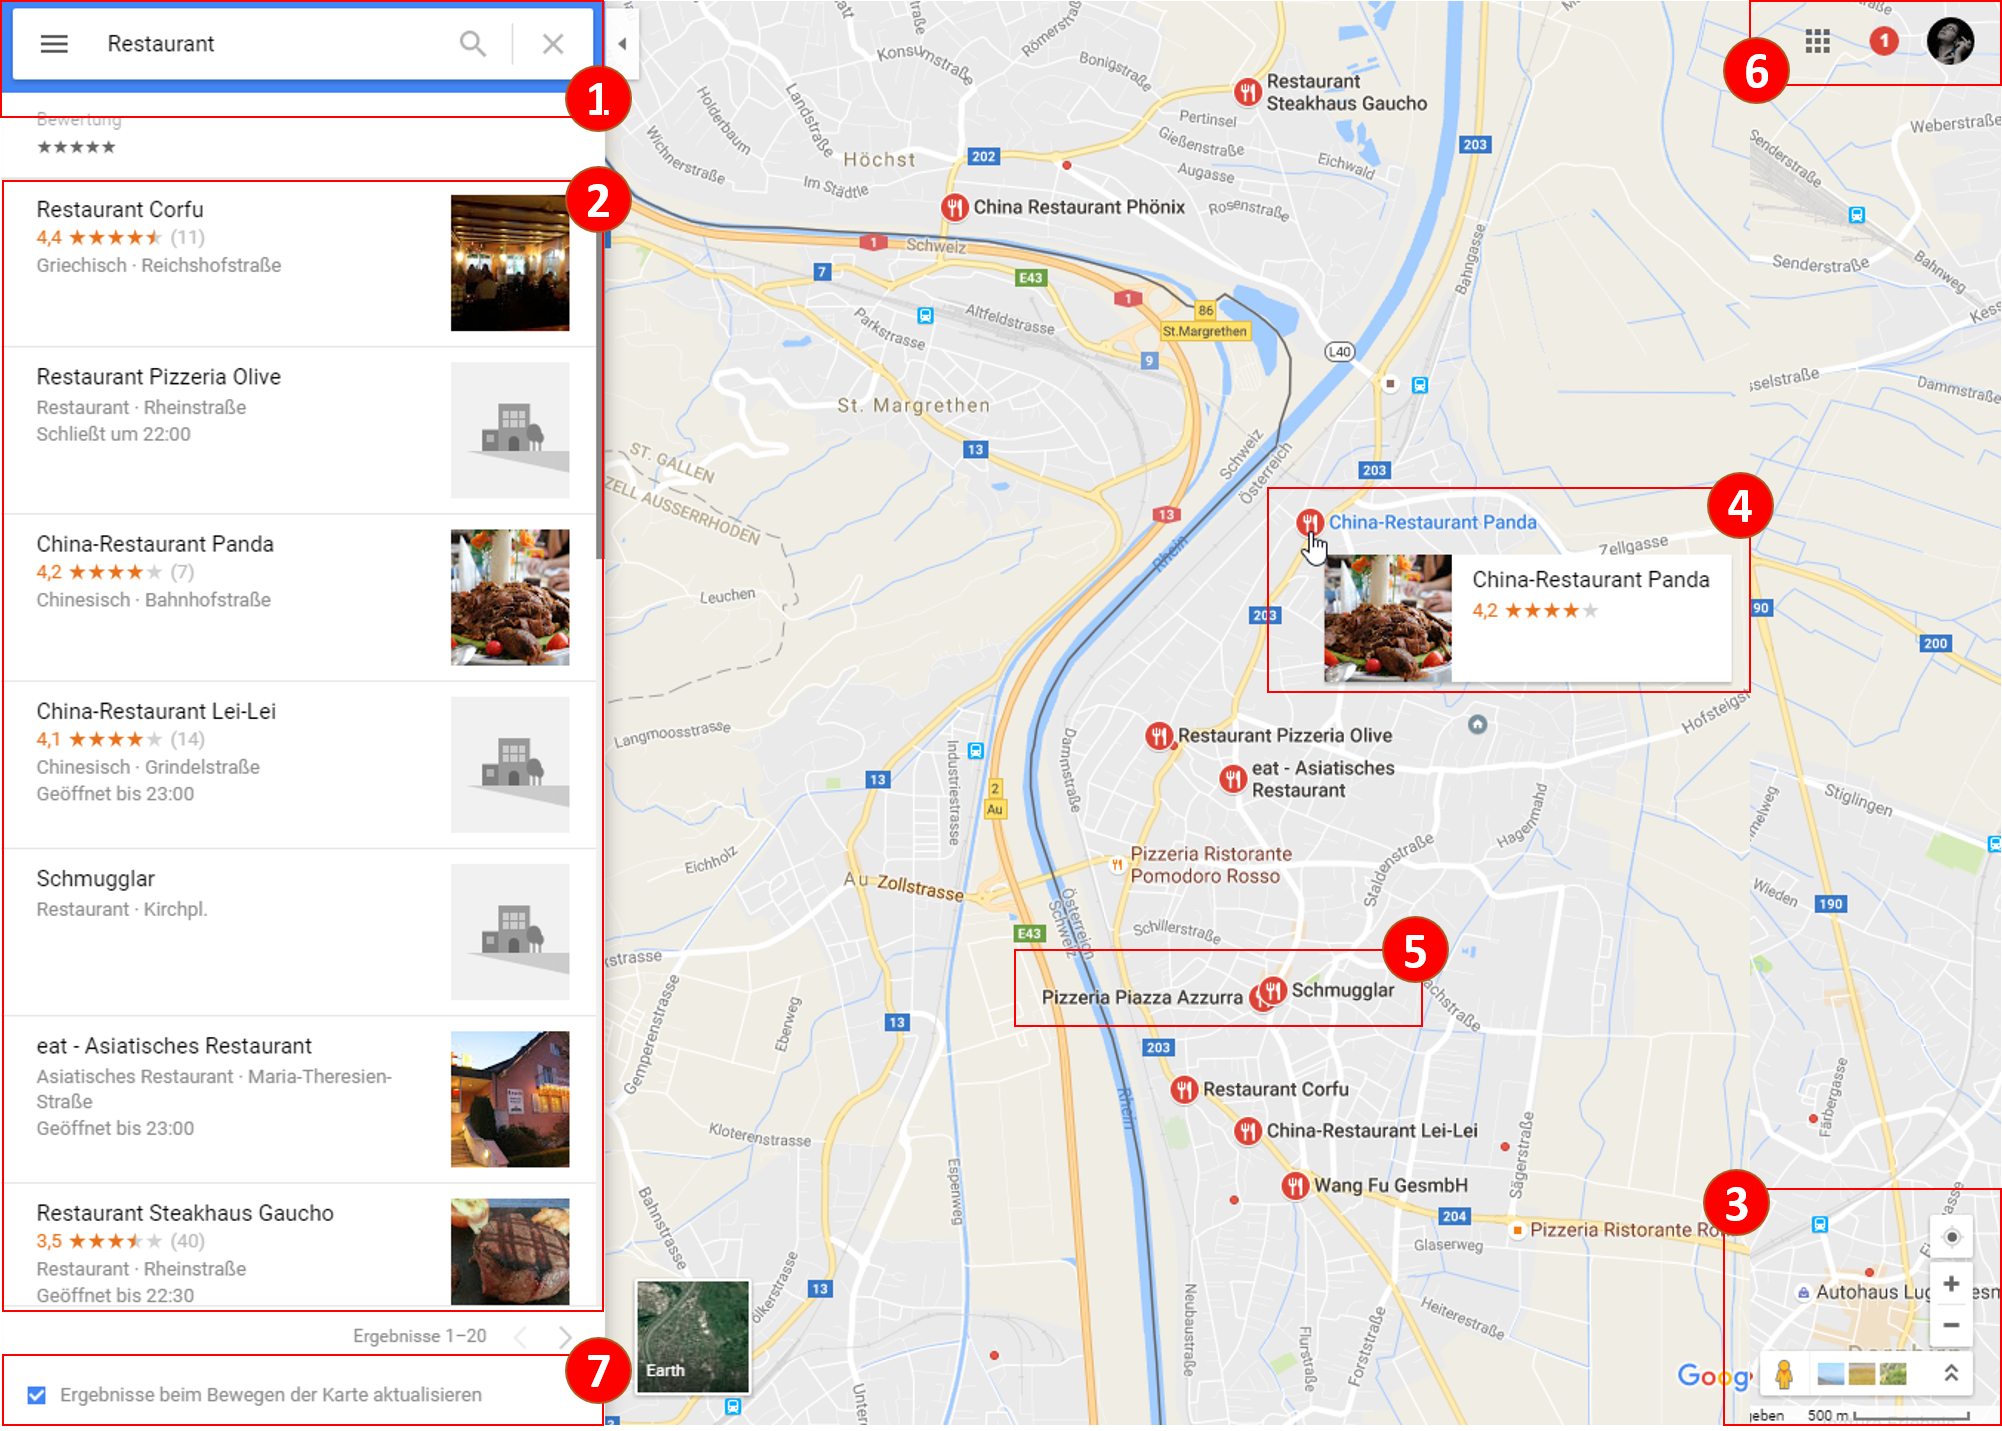
\includegraphics[width=1\linewidth]{img/StandDerTechnik/googlemapOverview}
\caption[Übersicht: Aufbau von Google Maps]{Übersicht: Aufbau von Google Maps. Bei der Abb.: handelt es sich um eine bearbeitet Version des Screenshots. Aus Gründen der Übersichtlichkeit wurde ein Teil der Kartenbereichs entfernt (Quelle: eigene Ausarbeitung | Daten und Kartenmaterial: https://www.google.at/maps/ - Stand Sommer 2016)}
\label{fig:googlemapOverview}
\end{figure}

\subsection{Zusammenfassung Google Maps}
Google Maps ist schlicht und übersichtlich gehalten.
Sämtliche Filter- und Anreicherungseinstellungen sind durch die ausklappbaren Menüs in den Hintergrund gewandert.
Dies wirkt sehr aufgeräumt und geradlinig allerdings führt es auch dazu, dass man gewisse Einstellungen nicht sofort findet.
Ein Beispiel bei dem mir dieses Problem im Zuge der Recherche aufgefallen ist war die Option die aktuelle Verkehrslage in der Karte einzublenden.
Diese Option versteckt sich hinter dem Menü-Button der Suchleiste (siehe Abb.: \ref{fig:googlemapOverview}-1). 
Was uns zum nächsten Punkt führt, dass ich an dieser Stelle Schamber recht geben kann das der Button durch das Hamburger-Design, ohne Rahmen oder eine sonstige optische Abgrenzung, schlecht als Schaltfläche zu erkennen ist (vgl.: \cite{SchamberHamburgerIcon}).\\
\\
Des weiteren verfolgt Google Maps den Ansatz die Informationen auf verschieden Arten zu visualisieren. 
Sehr interessant ist dabei die Verknüpfung zwischen der \nameref{gmapsList} und \nameref{gmapsMap}, die hier sogar in beide Richtungen funktioniert\footnote{sobald die Option Ergebnisse beim Bewegen der Karte aktualisieren aktiviert ist (siehe Abb.: \ref{fig:googlemapOverview}-5)}.\\
\\
Ein weiterer Punkt der für mich in der Kartendarstellung etwas verwirrend war ist die Frage warum manche Ergebnisse als größeres Icon mit Beschriftung und andere Ergebnisse als kleinerer roter Punkt ohne Beschriftung dargestellte werden. 
Zusätzlich zu der Größe werden die kleineren Punkte von den größeren Punkten überlagert wenn man die Zoomstufe ändert (siehe Abb.: \ref{fig:googlemapDetail})


\begin{figure}[H]
\centering
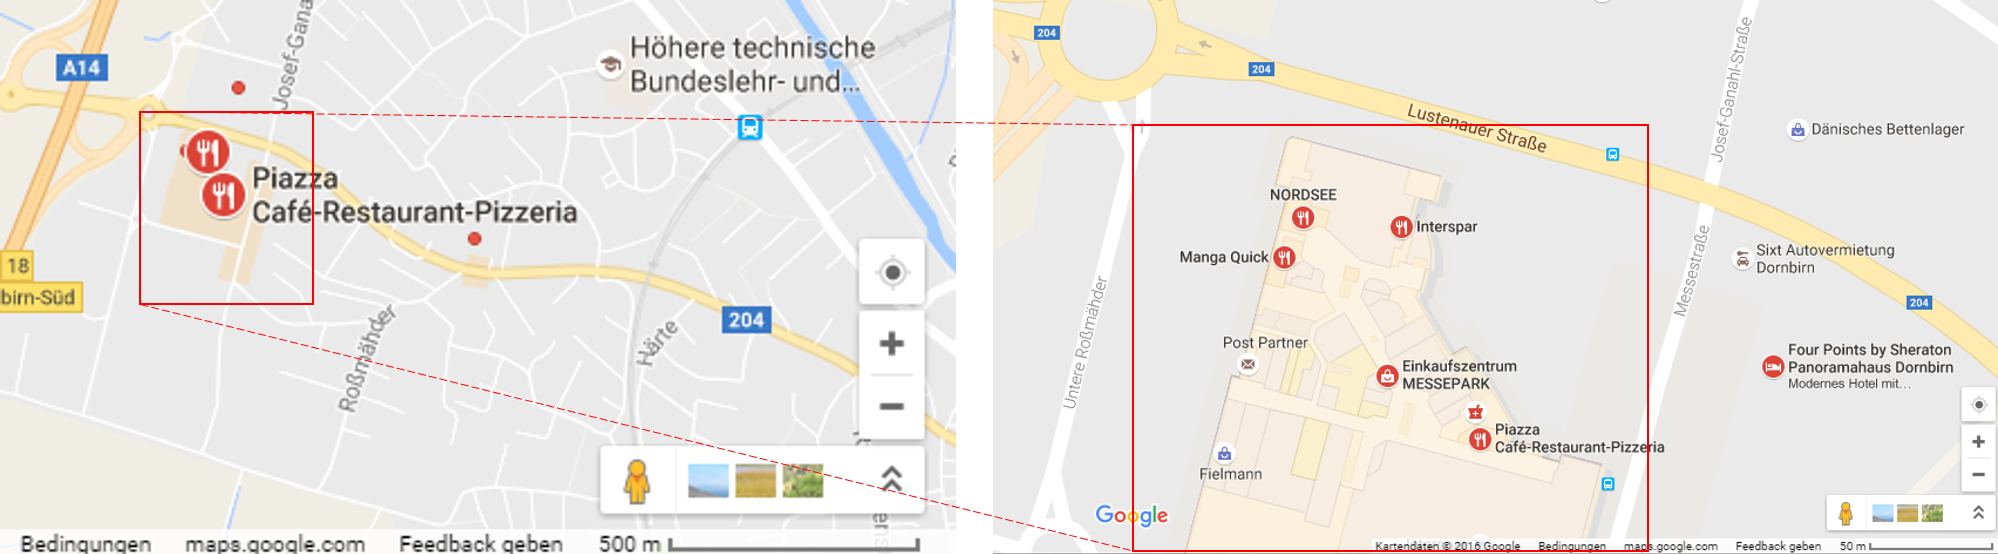
\includegraphics[width=1\linewidth]{img/StandDerTechnik/googlemapDetail}
\caption[Details: Überlagerung von Markierungen auf Google Maps]{Details: Überlagerung von Markierungen auf Google Maps. Der linke Kartenausschnitt zeigt eine Vergrößerung um den Faktor Zehn gegenüber dem rechten Kartenausschnitt. Der rote Rahmen markiert das jeweils das gleiche Gebäude. (Quelle: eigene Ausarbeitung | Daten und Kartenmaterial: https://www.google.at/maps/ - Stand Sommer 2016)}
\label{fig:googlemapDetail}
\end{figure}


Füge einen fehlenden Ort hinzu

\section{Airbnb}
\label{Airbnb}
Bei Airbnb handelt es sich um eine Webseite die sich auf die Vermittlung von Unterkünften spezialisiert hat\footnote{
	Airbnb ist unter der Adresse https://www.airbnb.com/ zu erreichen.
	}. 
Dabei können sich gastgebende Personen registrieren und Übernachtungsmöglichkeiten von einem Zimmer bis hin zu ganzen Immobilien anbieten. 
Anhand diverser Such- und Filterkriterien ermöglicht die Webseite den Suchenden eine passende Unterkunft zu suchen und diese über die Webseite zu reservieren.
Neben klassischen Bewertungen bietet die Webseite auch Social Media Komponenten wie Profile, das hochladen eigener Fotos und das liken  sowie die Möglichkeit sich als gastgebende Person eine eigene Marke aufzubauen (vgl. \cite{Yannopoulou2013}, S. 3).

\subsection{Aufbau von Airbnb}
Nachdem auf der Startseite die gewünschte Stadt in der man übernachten möchte, sowie optional das Start- und das Enddatum, ausgewählt wurden wird man auf die eigentliche Seite zur Planung weitergeleitet (siehe Abb.: \ref{fig:airbnbOverview}).
Die Planungsansicht unterteilt sich in die drei Bereiche \nameref{airbnb:filter}, \nameref{airbnb:gridview} sowie der \nameref{airbnb:map}.
Die jeweiligen Bereiche sind durch unterschiedliche Farbgebungen des Hintergrundes klar voneinander abgetrennt.

\paragraph{Auswahlkriterien/Filter}
\label{airbnb:filter}
Die Ansicht des Bereichs \nameref{airbnb:filter} kann der Abb.: \ref{fig:airbnbOverview}-1 entnommen werden (links oben).
Durch Änderungen in diesem Bereich werden die beiden anderen Bereiche (\nameref{airbnb:gridview} und \nameref{airbnb:map}) automatisch aktualisiert. 
Dieser Bereich ist in der Standardansicht in vier Zeilen aufgeteilt. 
In der ersten Zeile (ganz oben) befindet sich ein Textfeld welches Standardmäßig die zuvor ausgewählte Stadt/Region anzeigt. 
Sobald man das schreiben im Textfeld beginnt, wird man bei der Eingabe durch eine Auswahl passender Einträge unterstützt, welche unter dem Textfeld eingeblendet werden.
Mithilfe der zweiten Zeile von oben lassen sich die optionalen Daten von der Startseite (Start-, Enddatum und Anzahl der Gäste) nachtragen oder ändern.
Die Art der Unterkunft wird mit Hilfe der dritten Zeile von oben ausgewählt.\\
\\
In der vierten Zeile von oben werden die Preise mit Hilfe eines stilistischen Balkendiagramms angezeigt. Dabei verlaufen die Preise ansteigend auf der X-Achse.
Die Information über die Anzahl der Unterkünfte in der entsprechenden Preisklasse wird mithilfe der Y-Achse schematisch dargestellt
\footnote{Die genau Information kann aufgrund der fehlenden Beschriftung der Y-Achse oder einer anderen visuellen Unterstützung nicht abgelesen werden.
	}.
Mithilfe von zwei Schiebereglern kann die untere- und obere Grenze für die Preisspanne festgelegt werden, der jeweilige Betrag wird direkt unter den Reglern dargestellt.
Zusätzlich wird der durchschnittliche Preis der Region/Stadt unter der Preisspanne dargestellt.\\
\\
Mit einem klick auf den Button Filter (siehe Abb.: \ref{fig:airbnbOverview} - linke Seite zwischen oberen- und unteren roten Rahmen) wird der Bereich \nameref{airbnb:filter} expandiert und überlagert die  \nameref{airbnb:gridview}.
Dabei ist aufgefallen das die Platzierung des Buttons für mich etwas irritierend wirkt. 
Wie zuvor erwähnt, werden die einzelnen Bereiche durch die unterschiedliche Farbgebung des Hintergrundes abgegrenzt. 
Dabei befindet sich der Button Filter im grauen Bereich (\nameref{airbnb:gridview}) wenn man allerdings darauf klickt wird der expandierte Bereich in der hellen Hintergrundfarbe des \nameref{airbnb:filter}-Bereichs dargestellt.


\paragraph{Rasterdarstellung}
\label{airbnb:gridview}
Die Ansicht des Bereichs \nameref{airbnb:gridview} kann der Abb.: \ref{fig:airbnbOverview}-2 entnommen werden (links unten).
Die Ergebnisse der Einstellungen, welche im Bereich \nameref{airbnb:filter} getroffen wurden, werden hier in Form von Kacheln in einer Rasteransicht dargestellt.
Dies ist der einzige Bereich der über eine Scroll - Funktionalität verfügt.
Den Hintergrund von jedem Ergebnis stellt ein Bild der Unterkunft da. 
Durch die eingeblendeten Steuerelement
	\footnote{Die Steuerelemente werden eingeblendet sobald man mit dem Cursor über das Bild geht.} 
kann das Hintergrundbild durch andere Bilder aus der jeweiligen Galerie ersetzt werden. 
Des Weiteren werden neben dem Preis und des Profilbildes der gastgebenden Person auch die zusammengefassten Informationen der Unterkunft dargestellt. 
Mit einem klick auf Bild öffnet sich die entsprechende Detailseite der Unterkunft. 

\paragraph{Kartendarstellung}
\label{airbnb:map}
Die Ansicht des Bereichs \nameref{airbnb:map} kann der Abb.: \ref{fig:airbnbOverview}-3 entnommen werden (rechts).
Dieser Bereich unterstützt die Anwenderinnen bei der geografischen Orientierung dadurch, das die gleichen Ergebnisse wie im Bereich \nameref{airbnb:gridview} auf einer Karte visualisiert werden.
Dabei wird jede Unterkunft als eine eigenständige Markierung dargestellt, welche mit dem jeweiligen Preis versehen ist.
Durch einen klick auf die Markierung öffnet sich ein Popup, in welchem ein Bild der Unterkunft
\footnote{
	Auch hier gibt es im Popup die Möglichkeit sich durch die Galerie zu bewegen (siehe Absatz: \nameref{airbnb:gridview}).
	} 
sowie der Preis und weitere Informationen dargestellt werden. 
Wie auch im Absatz \nameref{airbnb:gridview} beschrieben lässt sich die Detailseite der Unterkunft über einen klick auf das Bild öffnen.
Die Farbgebung der Karte selbst ist dezent gehalten was wiederum die Sichtbarkeit der Markierungen erhöht.
Eine zusätzliche Farbcodierung von Informationen ist dabei nicht angedacht, alle Markierungen sind gleich eingefärbt.
Allerdings wechselt eine Markierung die Farbe (von rot nach grau) sobald man auf ihn geklickt hat und das erscheinende Popup wieder schließt.
Markierungen sich auf Grund der Zoomstufe überlagern werden nicht gesondert dargestellt.

\begin{figure}[H]
	\centering
	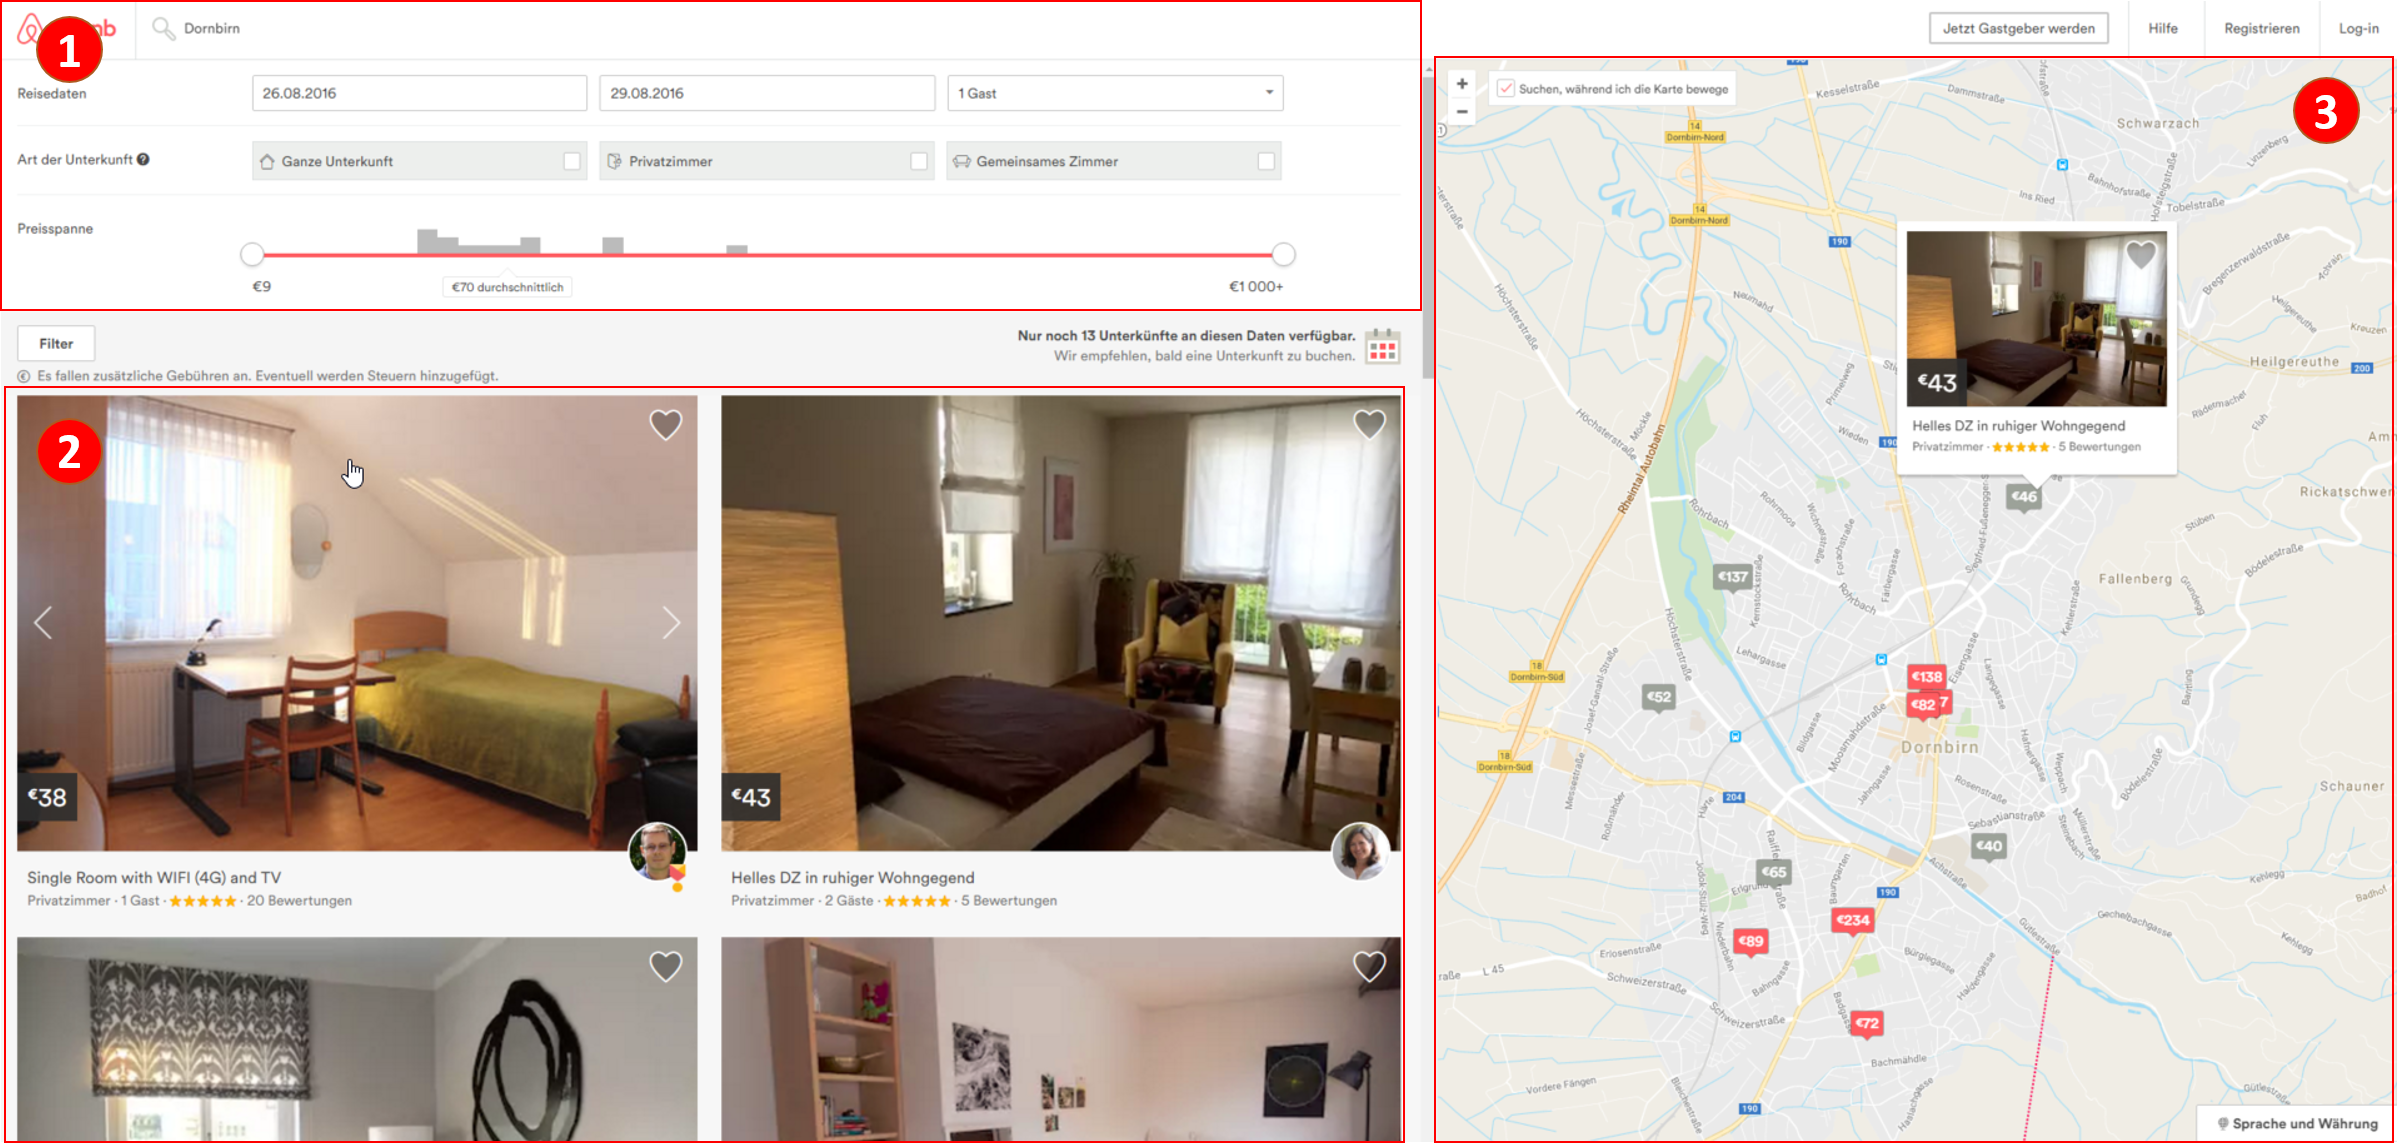
\includegraphics[width=1\linewidth]{img/StandDerTechnik/airbnbOverview}
	\caption[Übersicht: Aufbau von Airbnb]{Übersicht: Aufbau von Airbnb (Quelle: eigene Ausarbeitung | Daten und Kartenmaterial: https://www.airbnb.com/ - Stand Sommer 2016)}
	\label{fig:airbnbOverview}
\end{figure}

\subsection{Zusammenfassung Airbnb}
\label{airbnb:review}
Die Auswahlseite ist schlicht und übersichtlich gehalten wodurch die einzelnen Bereiche schnell identifiziert werden können, mit Ausnahme des Filter-Buttons (siehe Absatz: \nameref{airbnb:filter}). 
Die Funktionalität des Preisspannen Filters ist aus meiner Sicht sofort erkenntlich gewesen und bietet auf den ersten Blick eine gute Übersicht über die Preisverteilung der Unterkünfte.
Etwas unübersichtlich ist die \nameref{airbnb:map}, sobald mehrere Markierungen nebeneinander liegen wodurch diese (abhängig von der Zoomstufe) überlagert werden und der beschriftete Preis nicht mehr ersichtlich ist. \\
\\
Sehr interessant ist die Idee, die Ergebnisse auf zwei verschiedene Arten zu visualisieren (die Bereiche \nameref{airbnb:gridview} und \nameref{airbnb:map}).
Dies ermöglicht eine Auswahl nach der geografischen Lage (\nameref{airbnb:map}) sowie nach den Bilder der Unterkunft beziehungsweise den weiteren Informationen in der \nameref{airbnb:gridview}
Zusätzlich wurden die beiden Bereiche miteinander verknüpft. 
Sobald man mit der Maus ein Bild in der \nameref{airbnb:gridview} berührt wird die zugehörige Markierung auf der Karte dunkelgrün hervorgehoben (siehe Abb.: \ref{fig:airbnbDetail} wodurch das abwechselnde Arbeiten in beiden Bereichen vereinfacht wird.


\begin{figure}[H]
\centering
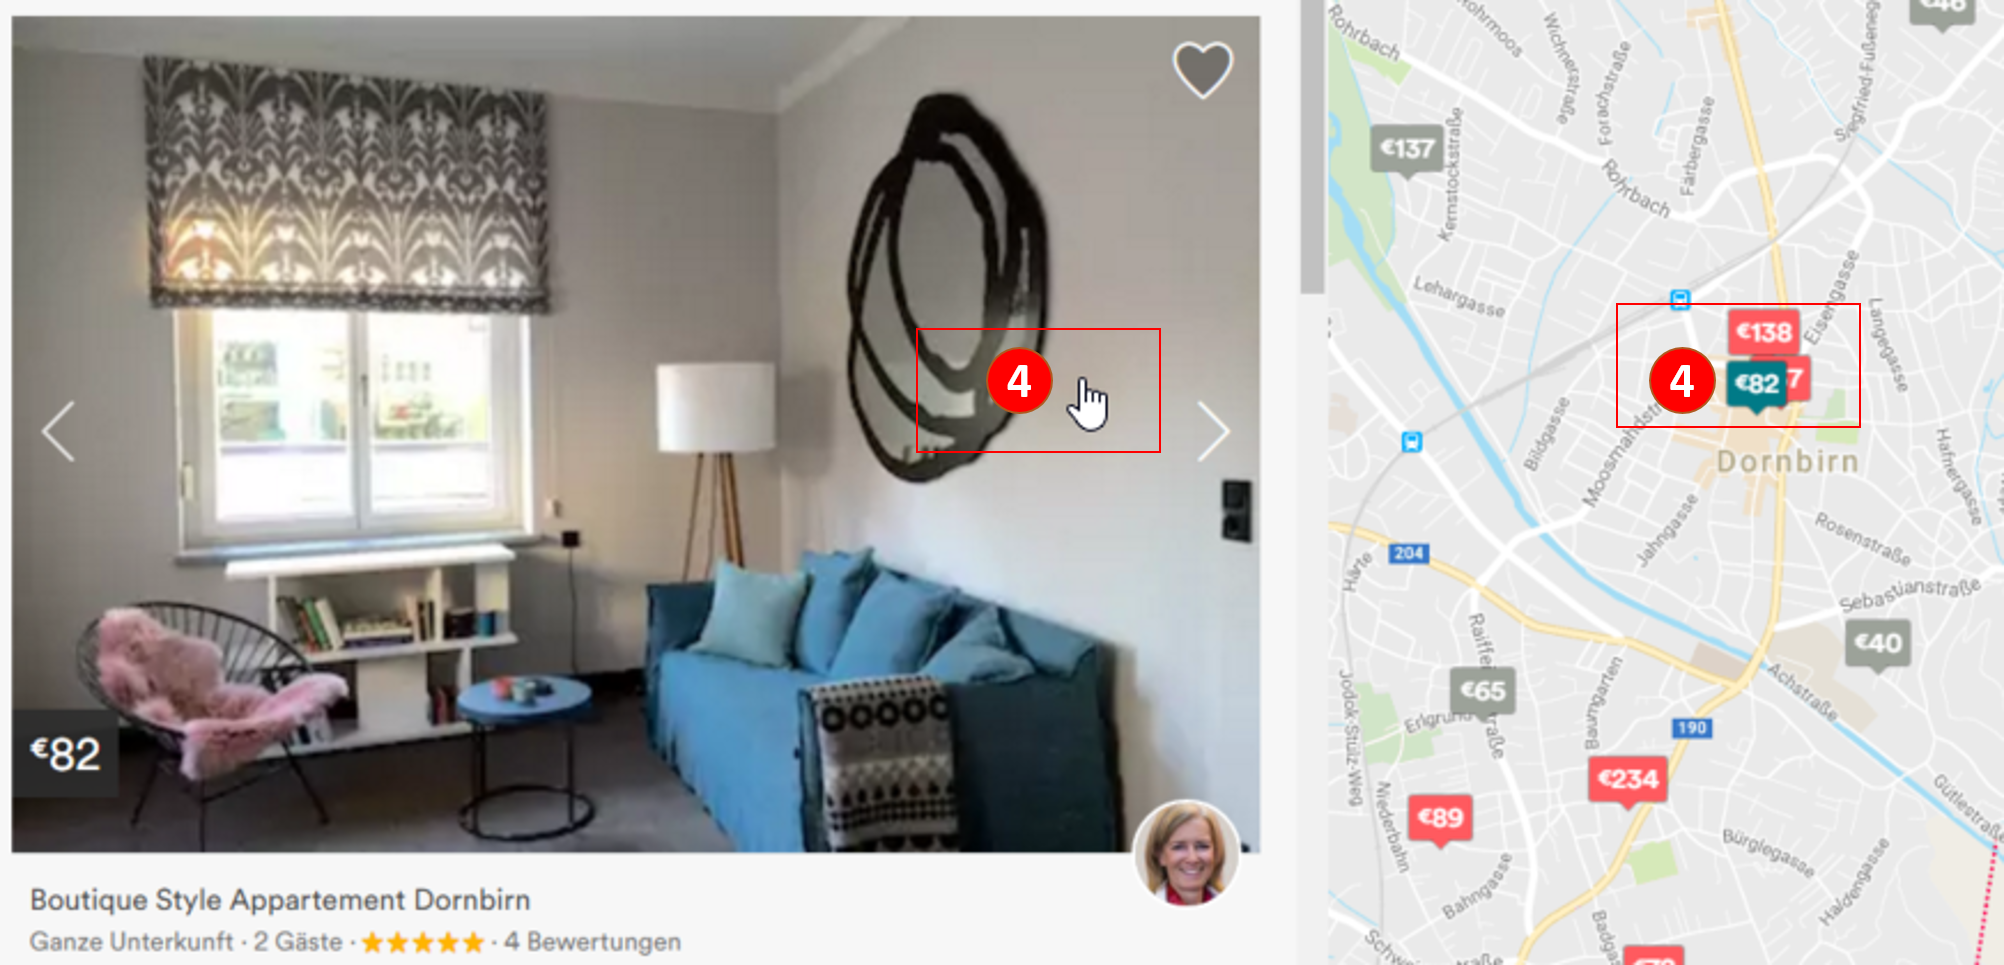
\includegraphics[width=1\linewidth]{img/StandDerTechnik/airbnbDetail}
\caption[Verknüpfung der Raster- und Kartenansicht]{Verknüpfung der Raster- und Kartenansicht (Quelle: eigene Ausarbeitung | Daten und Kartenmaterial: https://www.airbnb.com/ - Stand Sommer 2016)}
\label{fig:airbnbDetail}
\end{figure}




\section{Flightradar24}
\label{Flightradar}
Bei Flightradar24 handelt es sich um eine Webseite die Live-Daten des Internationalen Flugverkehrs speichert und visualisiert. 
Um die Daten zu erfassen nutzt Flightradar24 Empfangsstationen am Boden die das Signal der in den Flugzeugen befindlichen Transponder auffängt und in die Datenbanken von Fligthradar24 einspeist. 
Beim Absturz der Gemaanwings-Maschine 9525 unterstützte der Service erfolgreich die Rettungsgruppen bei der Ortung des Unglücksorts in Südfrankreich (vgl.: \cite{SiebeckFlightradar}).


\subsection{Aufbau von Flightradar24}
\label{flightradarAufbau}
Im Gegenteil zu den beiden vorherigen Seiten wirkt Flightradar24 auf den ersten Blick unübersichtlich und durch die sich in Echtzeit bewegenden Flugzeugmarker unruhig (siehe Abb.: \ref{fig:flightradarOverview}).
Die Seite selbst ist in eine Navigationsleiste (siehe Abb.: \ref{fig:flightradarOverview}-1), eine Detailansicht (siehe Abb.: \ref{fig:flightradarOverview}-2) und die Kartenansicht mit den Einstellungsmöglichkeiten und dem Suchfeld in einem halb-transparenten Overlay unterteilt (siehe Abb.: \ref{fig:flightradarOverview}-3). 


\begin{figure}[H]
\centering
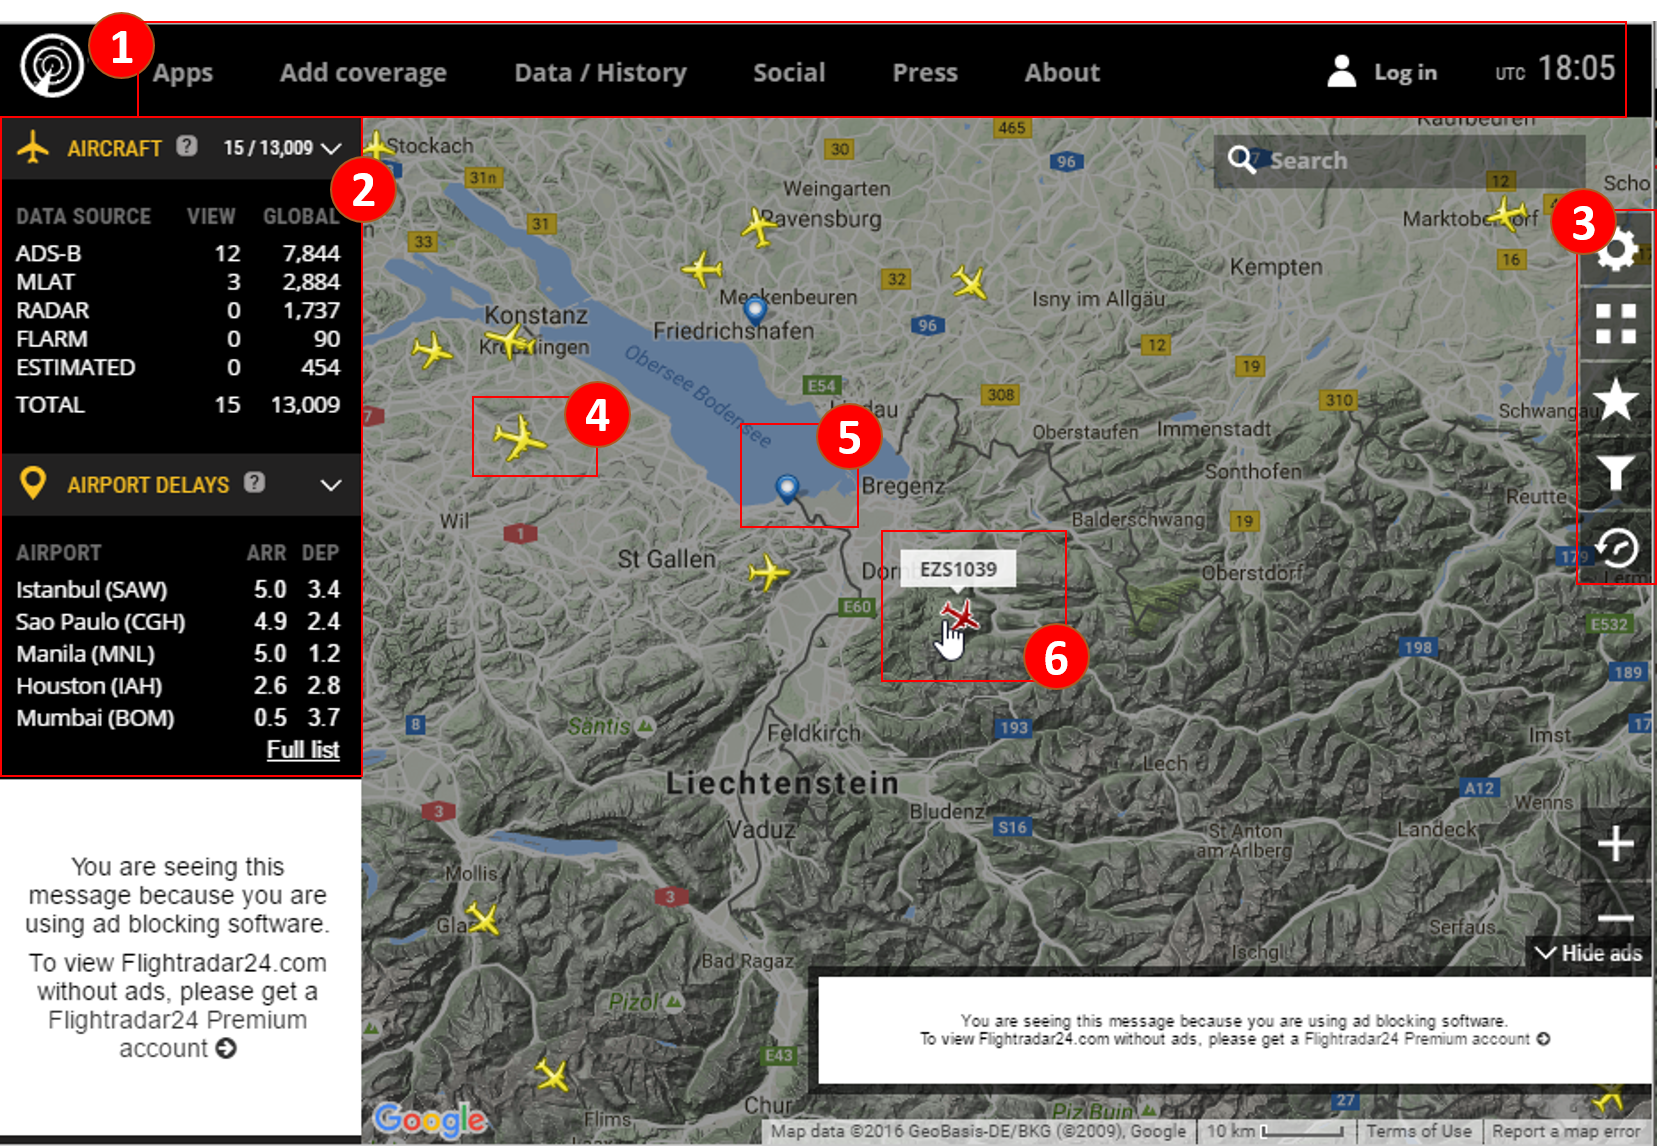
\includegraphics[width=1\linewidth]{img/StandDerTechnik/flightradarOverview}
\caption[Übersicht: Aufbau von Flightradar24]{Übersicht: Aufbau von Flightradar24 (Quelle: eigene Ausarbeitung | Daten und Kartenmaterial: https://www.flightradar24.com - Stand Sommer 2016)}
\label{fig:flightradarOverview}
\end{figure}

\paragraph{Suchfeld}
Das Suchfeld ist in der rechten oberen Ecke (siehe Abb.: \ref{fig:flightradarOverview}) und wurde von mir als Teilbereich der Kartendarstellung wahrgenommen\footnote{Im Gegensatz zu beiden anderen Webseiten bei der das Suchfeld im linken oberen Bereich, klar getrennt von dem Kartenbereich, platziert ist.}. 
Die Suche hat in dieser Applikation den primären Zweck einzelne Objekte (wie beispielsweise Flugzeuge oder Flughäfen) zu finden und nicht Region oder Städte.\\
\\
Die Suchergebnisse werden nicht in einem separaten Bereich sondern direkt unter dem Suchfeld angezeigt, welches sofort beim tippen die Ergebnisse darstellt.  
Dabei werden die Ergebnisse nach Kategorie, wie beispielsweise Flughafen oder Flug, gruppiert und nur eine überschaubare Anzahl an Treffern dergestalt mit dem Hinweis das mehr Treffer abgerufen werden können.
(siehe Abb.: \ref{fig:flightradarDetail}-7)

\paragraph{Kartendarstellung}
\label{flightradarMap}
Wie Eingangs erwähnt teilt sich die Kartendarstellung den Platz im Darstellungsbereich mit der diversen Optionsmenüs (siehe Abb.: \ref{fig:flightradarOverview}-3). 
Beispielsweise kann über das Zahnrad-Symbol ein verschachteltes Menü mit diversen Karten-, Wetter- und Layereinstellungen aktiviert werden (siehe Abb.: \ref{fig:flightradarDetail}-8).\\
\\
Auf der Karte selbst werden zwei Arten von Markern eingesetzt. 
Zum einen Flugzeuge und zum anderen klassische Pins für die Visualisierung von Flughäfen.
Dabei ist bei beiden Arten keine farbige Kodierung von Informationen vorgesehen, allerdings unterscheiden sich die Marker der Flugzeuge in der Größe von einander (siehe Abb.: \ref{fig:flightradarOverview}-4 und \ref{fig:flightradarOverview}-5).\\
\\
Sobald ein Flugzeug- oder eine Flughafen mit der Maus berührt wird erscheint ein Popup das ausschließlich den Namen des Flughafens beziehungsweise die Rufkennung des Flugzeugs einzeilig in reiner Textform darstellt.
Etwas inkonsistent verhält sich die Webseite sobald man auf einen Marker klickt.
Im Fall eines Flugzeuges wird der Bereich der linken Seite (siehe Abb.: \ref{fig:flightradarOverview}-2) durch eine Detailansicht des entsprechenden Flugzeuges ersetzt (siehe Abb.: \ref{fig:flightradarDetail}-9).
Anders verhält sich die Webseite wenn man auf einen Flughafen klickt, in dem Fall wird die gesamte Webseite durch die Detailseite des Flughafens ersetzt von der aus man nicht mehr durch einen Link oder die Browsernavigation zurück zur Kartenansicht gelangt.

\paragraph{Detaildarstellung}
\label{flightradarDetaildarstellung}
Nachdem die Seite geladen ist wird dieser Bereich zum einen dafür verwendet um relevante Informationen anzuzeigen wie Beispielsweise die Datenquellen und aktuelle Verspätungen auf Flughäfen und zum anderen weniger relevante Informationen wie zum Beispiel die aktuelle Tweets und Blog Posts des Unternehmens sowie Werbung für die eigenen Apps (siehe Abb.: \ref{fig:flightradarOverview}-2). 
Sobald man allerdings auf einen Flugzeugmarker klickt, wird die Ansicht mit der Detailansicht des entsprechenden Fluges ersetzt (siehe Abb.: \ref{fig:flightradarDetail}-9).\\
\\
Während die Informationen in den Popups über den Flugzeugmarkern eher von minimalistischer Natur sind fallen die visualisierten Informationen zum Flug im linken Seitenbereich sehr detailliert und übersichtlich aus (siehe Abb.: \ref{fig:flightradarDetail}-9). 
Der Detailbereich ist dabei in unterteilt in Flugstatus, Flugzeugdetails und Flugdetails.
In der Gruppe Flugstatus lässt sich sofort erkennen wo der Flug wann gestartet ist und wann er wo planmäßig landen wird, zusätzlich wird die aktuell zurückgelegte Flugstrecke anhand eines Zeitstrahls dargestellt.
Ein klick auf den Start- und Zielflughafen öffnet direkt die entsprechende Detailansicht.
Zusätzlich werden die aktuellen Koordinaten sowie das lokale Wetter des Fluges in der Gruppe Flugdetails angezeigt. 

\begin{figure}[H]
\centering
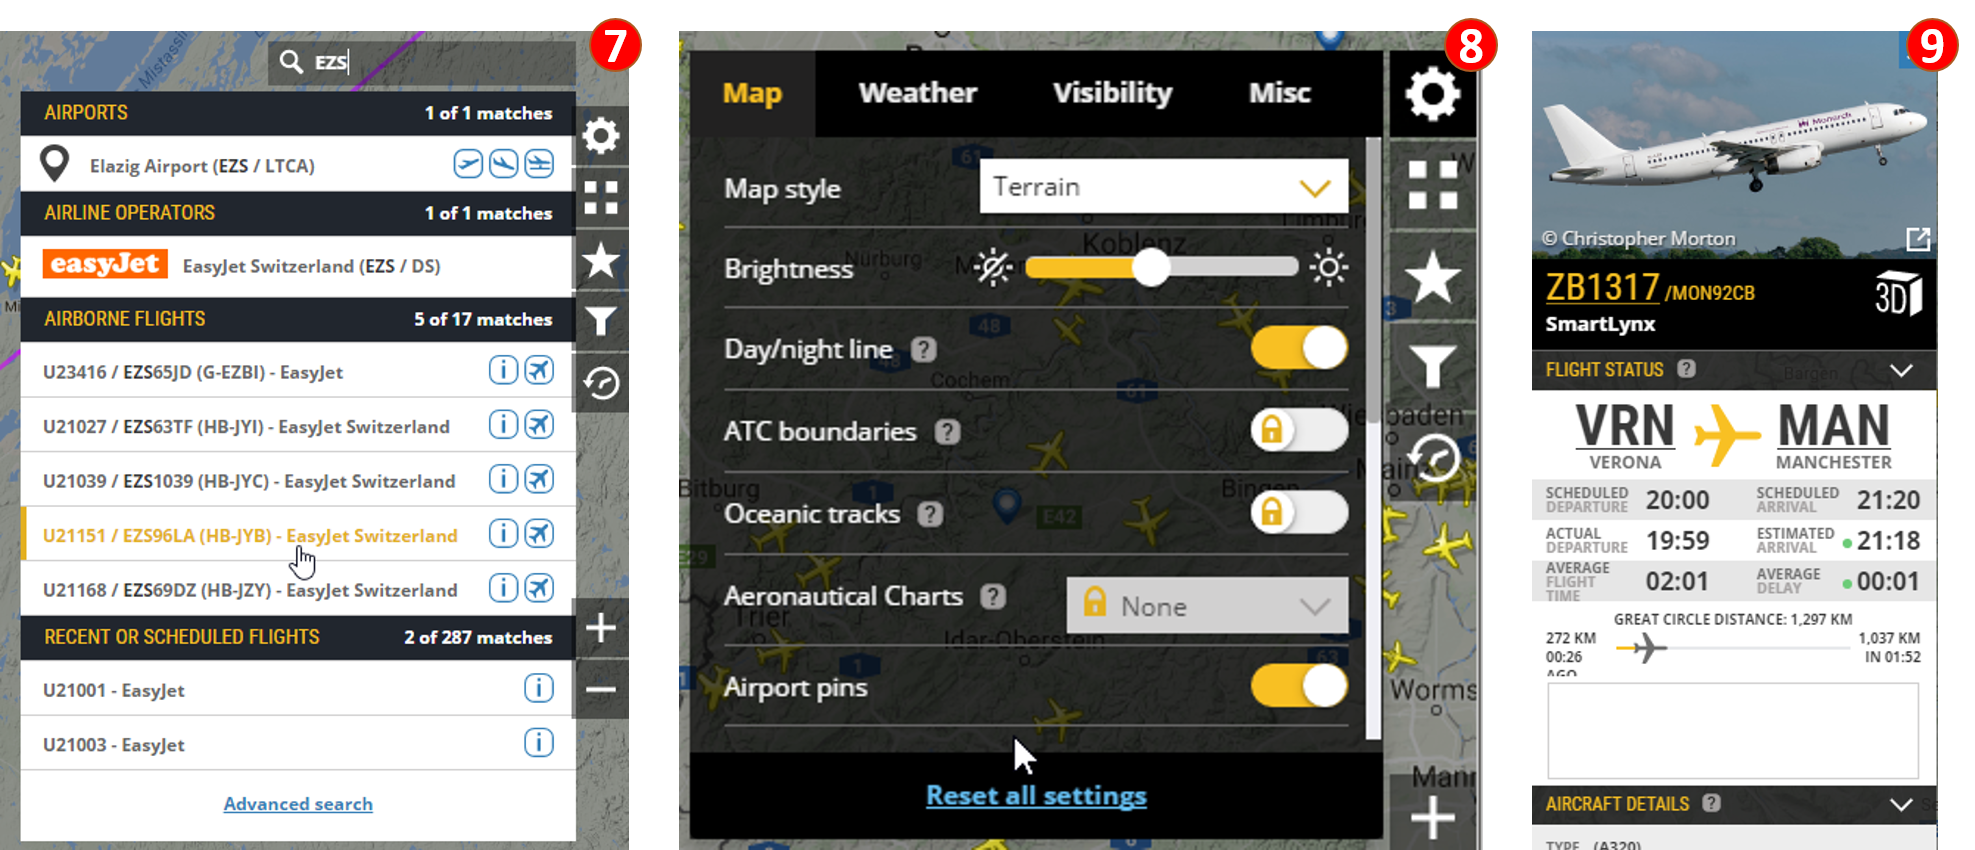
\includegraphics[width=1\linewidth]{img/StandDerTechnik/flightradarDetail}
\caption[Details: Flightradar24]{Details: Flightradar24. 7: Ansicht der Suchfunktion, 8: Ansicht der Optionen, 9: Detailansicht eines Fluges (Quelle: eigene Ausarbeitung | Daten und Kartenmaterial: https://www.flightradar24.com - Stand Sommer 2016)}
\label{fig:flightradarDetail}
\end{figure}


\subsection{Zusammenfassung Flightradar24}
Wie zuvor erwähnt empfinde ich den Aufbau der Seite als Überladen und schwer (siehe Absatz: \nameref{flightradarAufbau}). 
Dies liegt zum einen an der dunkel gehaltenen Farbgebung der Seite und zum anderen daran das (aus meiner Sicht) zu viele relevante sowie weniger relevante Informationen dargestellt werden.
Beispielsweise hat die Navigationsleiste (siehe Abb.: \ref{fig:flightradarOverview}-1) keine relevante Funktion für meine Recherchen bereitgestellt. 
Das gleiche betrifft den unteren linken Bereich in dem die aktuellen Tweets und Blog Posts des Unternehmen dargestellt werden (siehe Absatz: \nameref{flightradarDetaildarstellung}). 
Zusätzlich fand ich das inkonsistente Verhalten beim klicken auf eine Kartenmarkierung verwirrend. 
Wie im Absatz \nameref{flightradarMap} beschrieben verhält sich die Seite unterschiedlich je nach dem ob man auf ein Flugzeug oder einen Flughafen klickt.\\
\\
Aus meiner Sicht ist die Karte im normalen Zustand zu Farbintensiv, dies lässt sich allerdings individuell in den Option einstellen und beispielsweise in Grautöne abändern.
Sehr interessant ist die Art und Weise wie die detaillierten Informationen zu einem speziellen Flug übersichtlich und klar visualisiert werden.

\section{Ergebnisse der Analyse}
Zum Abschluss der Analyse sollen an dieser Stelle die Konzepte und Inspirationen aufgezeigt werden welche in den einzelnen Webseiten entdeckt wurden und als Mehrwert in das Konzept mit einfließen werden.

\begin{enumerate}
	\item Allgemein
	\begin{enumerate}
		\item[] Eine übersichtliche und helle der Darstellung wie am Beispiel von \nameref{chap:analyse:sec:sota:sec:google_maps} und \nameref{Airbnb}.
		\item[] Verschiedene miteinander verknüpfte Darstellungsformen anbieten wie beispielsweise eine Listen- und eine Kartendarstellung (Beispiel: \nameref{chap:analyse:sec:sota:sec:google_maps} und \nameref{Airbnb}).
		\item[] Auf gute Erkennbarkeit von Buttons und Menüs achten (negativ Beispiel: \nameref{chap:analyse:sec:sota:sec:google_maps} - Menü-Button in der Suchleiste)
	\end{enumerate}
	\item Kartendarstellung
	\begin{enumerate}
		\item[] Eine dezente Farbgebung der Karte (\nameref{chap:analyse:sec:sota:sec:google_maps} und \nameref{Airbnb}).
		\item[] Gleichbehandlung von Markierungen auf der Karte (negativ Beispiel: \nameref{chap:analyse:sec:sota:sec:google_maps}).
		\item[] Auf konsistentes Verhalten bei unterschiedlichen Kartenmarkierungen achten (negativ Beispiel: \nameref{Flightradar}).
	\end{enumerate}
	\item Detailansicht
	\begin{enumerate}
		\item[] Strukturiert die wichtigsten Informationen auf einer separaten Seite anzeigen, mit der Möglichkeit leicht wieder zurück zur Suche zu wechseln (Beispiel: \nameref{Airbnb} und \nameref{Flightradar}).
	\end{enumerate}
\end{enumerate}

\section{Technologien}
\ideas{Hier noch die Evaluation der Webtechnologien berschreiben: Google Maps Api, Leaflet, etc.}

\end{document}